\chapter{Background and literature review}\label{chapter:background}
\thispagestyle{chapterBeginStyle}
\label{theoretical-background}

\section{Representation learning}
\textit{Representation learning}, often referred to as \textit{feature learning}, is a set of machine learning approaches that allows for automatic feature detection from data. This is in contrast to manual feature extraction which, while takes advantage of the domain knowledge about data and human ingenuity, is both time-consuming, labor-intensive and cannot take advantage of the latent space. A comprehensible definition of representation learning was formulated by Bengio et al. \cite{Bengio2012} in 2012:

    \begin{definition}[Representation learning]\label{def:representation-learning}
    Learning representations of the data that make it easier to extract useful information when building classifiers or other predictors.
    \end{definition}
\autoref{def:representation-learning} does not, however, delve into the core issue of what the representation is – even though the definition seems to be intuitive, it is hardly to be found in the domain-specific literature.

\vspace{\baselineskip}
\subsection{What is a representation?}\label{subsec:representation}
As it often comes with Artificial Intelligence, being highly inspired by processes taking place in nature (in particular by the field of cognition, which is the main interest of cognitive science), it is not the sole domain whose interests revolve around representations. Not only the term itself, but also the very ontology of representations, play a central role in neuroscience literature. However, even there neither a clear consensus on all aspects, nor a unified definition of it exist \cite{Vilarroya2017}. Having said that, probably the most established is \autoref{def:representation-neuroscience}.

\begin{definition}[Representation (in neuroscience)]\label{def:representation-neuroscience}
A formal system for making explicit certain entities or types of information, together with a specification of how the system does this. \cite{Marr1982}
\end{definition}

An example of such would be a numeral system, which is a writing system for expressing (representing) numbers — the Roman, Hindu–Arabic (decimal) and binary being among the most widespread. \autoref{fig:numeric_systems} shows different representations of the same number in these systems.

% TODO: Create captions for particular representations.
% TODO: Improve main caption.
\begin{figure}[ht]
    \centering
    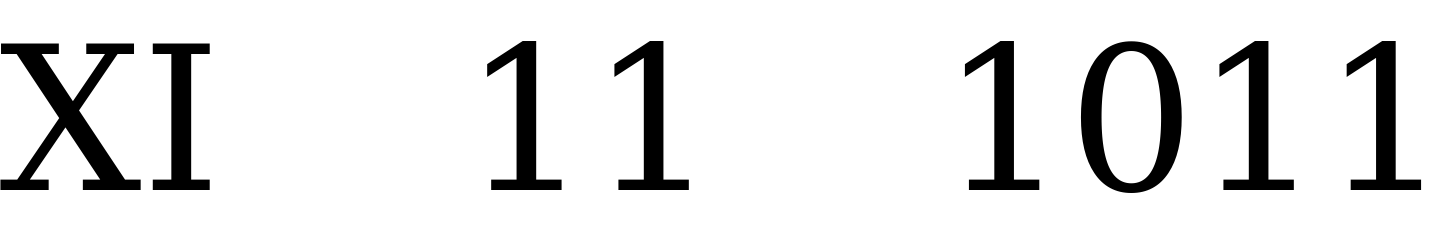
\includegraphics[width=0.8\textwidth]{background/images/numeric_systems.png}
    \caption[Numeric systems as representations]{Numeric systems as representations.}
    \label{fig:numeric_systems}
\end{figure}

% TODO: Find reference for decimal & binary being positional
% TODO: Find reference for binary being foundation of modern computing
Each of those representations was formed with a specific goal in mind – to simplify certain operations. The Roman system, used by the ancient Romans to count and perform other day-to-day transactions. It is non-positional \cite{Hazewinkel1990} and governed by principles of subtraction and addition. Despite being quite primitive, it had quickly become overcomplicated due to its poor scalability \cite{Ifrah1998}. It constituted a barrier to the mathematical development of the Roman Empire that had been significant to the earlier Arabic cultures. They had used the decimal numeric system, which, being multiplicative by nature (easily decomposed into powers of $10$) and positional, facilitates more complex arithmetics. The binary system, using only two symbols - $0$ and $1$ - through advancements of the Boolean algebra applied to the electrical switches, is widely used in modern computers. In general, each of them provides a different kind of abstraction to aid a specific objective.

\vspace{\baselineskip}
Despite the information content being the same in all three cases, their representation is different, which implies the orthogonality of the two. Switching between representations should not influence the original value they describe, and the transition process should be unambiguous due to explicitness (see \autoref{def:representation-neuroscience}). 
Even though systems might share the same symbols, values expressed by them might differ (i.e., a $1$ on $n$-$th$ position will produce a different value in decimal and binary system). Because of that, a representation should be defined by the shape of the manifold on which the data lie within the representational space, as opposed to a single piece of information \cite{Thompson2018}.

\vspace{\baselineskip}
According to the above, almost anything can be subject to being represented, from everyday objects to complex abstract concepts. Similarly, representation learning touches upon different aspects and applications of machine learning (for particular examples, see \autoref{sec:related-work}). A useful data representation should yield an improvement of the performance of a model, as well as facilitate the learning process – the scale of both highly depends on appropriately selected features (it is especially true for the deep learning models).
% TODO: Find why it is especially true for the deep models (literature).

\vspace{\baselineskip}
With this perspective, one could form a loose definition of \textit{representation} in machine learning:

\begin{definition}[Representation]\label{def:representation-ml}
A function mapping input data to a latent vector, which is useful for a task.
\end{definition}

Subsequently, \textit{representation learning} can be comprehended as an optimization problem of parameters of such function. If $x$ denotes the data, $\theta$ the parameters and $\vec{z}$ - the latent vector, the whole can expressed as \autoref{eq:representation-learning}.

\begin{equation}\label{eq:representation-learning}
    f\left(x;\theta\right)\rightarrow\vec{z}
\end{equation}
We expect the dimension of the representation to be not higher than the original data ($dim\left(\vec{z}\right) \le dim\left(x\right)$), but ideally it should be much lower ($dim\left(\vec{z}\right) \ll dim\left(x\right)$).


\subsection{What makes a good representation?}
According to \autoref{def:representation-ml}, the output set of features (ergo the latent vector) should be \textit{useful} for a specific \textit{task}. The task objective serves as a falsifiability mechanism defining their usefulness. It allows for eliminating uninformative features, and thus, reducing the dimensionality. The examples in \autoref{subsec:representation} emphasize the importance of a \textit{quality} representation. Hence, it is valid to ask: \say{\textit{what} makes a good representation?}. Surprisingly, it is an ill-defined and challenging question.


\subsubsection{Dimensionality reduction}
Yet again, cognitive science lays foundations for artificial intelligence and aids in answering fundamental questions. In 1959, Horace Barlow, identified the significance of \textit{redundancy reduction}\footnote{Barlow revisited the topic of redundancy reduction in 2001 \cite{Barlow2001}. He stated that \say{the original work was wrong in over-emphasizing the role of compressive coding and economy in neuron numbers, but right in drawing attention to the importance of redundancy}. Both documents accentuate the impact of Claude Shannon's work, as well as the \say{entanglement} and the mutual influence of neuroscience and artificial intelligence.} in information processing by human brains \cite{Barlow1959}. The original idea is to \say{achieve economy without losing any information at all}. It can be inexactly (representation learning usually assumes some information loss) translated to a dimensionality constraint defined along \autoref{eq:representation-learning}. Due to a threat of the \textit{curse of dimensionality}, it is desirable that the representation has minimal possible number of dimensions, while maintaining the variance level (at least for the data that is informative for the task at hand). Barlow's findings later became a base for research on disentangled representations. 


\subsubsection{Disentanglement}
The human perception of the world around heavily depends on visual recognition. Representations on the early stage of visual processing are not beneficial for the object recognition, because they are - \say{like two sheets of paper crumpled together} - \textit{tangled} \cite{DiCarlo2007}. Only at later stages it is being untangled \cite{DiCarlo2012}, therefore transformed from \say{visual representations that are easy to build, but are not easily decoded, into representations that we do not yet know how to build, but are easily decoded}.

\vspace{\baselineskip}
Correspondingly, building a solid representation for machine learning algorithms expects separation of information about the attributes (some features vary with respect to only one attribute), simplifying setting decision boundaries for subsequent tasks. Additionally, one wants to discard the build up of an unnecessary invariance related to nuisance attributes, but without disposing of practical information about the data. It diminishes the representation's sensitivity to the data's directions of variance that are not informative to the task. This procedure, called \textit{disentangling factors of variation} \cite{Szabo2017}, is nontrivial, but yields a representation, which is more robust than the original, tangled structure. 


\subsubsection{Geometric priors}
% TODO:
Despite real-world data often being incomplete (or even damaged), high-dimensional and chaotic, it often shows certain, usually hidden, regularities. A good representation should identify and capture them, ideally in a low-dimensional form. This limits the exponential space of possible functions. Such regularities can be exposed through unified geometric principles called \textit{geometric priors} \cite{Bronstein2021}. Two fundamental principles applied to physically structured data are scale separation and symmetry.

\vspace{\baselineskip}
\textit{Symmetry} of an object or a system is a transformation that leaves some property of the object or system unchanged or maintains its invariance. \textit{Scale separation}, on the other hand, retains important features of a signal during the transfer onto a coarser domain. 

\vspace{\baselineskip}
Invariance to scale, translation, or rotation often proves to be the key to improving performance of machine learning models. It is ubiquitous (and easily visualizable) in image processing. Convolutional Neural Networks, for instance, do incorporate the idea of geometric priors. Translational symmetry is achieved through filters with shared weights, while pooling exploits scale separation. They are not, however, fully invariant to rotation, unless appropriately extended.

\subsubsection{Smoothness}
Smoothness of the representation assumes its invariance to minor, insignificant changes of the data. Formally, it is expressed that if some input $x$ is approximately equal to some other input $y$ ($x \approx y$), the functions of both should also be approximately equal ($f(x) \approx f(y)$). It is one of the general priors, not only for representation learning, but also for the majority of machine learning approaches.

\vspace{\baselineskip}
Bengio et al. \cite{Bengio2012} argue that, while useful, this assumption alone is insufficient to overcome the \textit{curse of dimensionality} and \say{advocate learning algorithms that are flexible and non-parametric but do not rely exclusively on the smoothness assumption}.


\subsubsection{Distribution}
Distribution of a representation assumes spread of the representation's particular features across multiple parts of the same model — following the example of neural networks, the final feature value consisting of contributions from different neural paths. Moreover, it also induces feature abstraction and re-use, which facilitate utilization of simple representation to create more abstract ones in hierarchical models.


\subsection{Representation learning taxonomy}
%TODO introduce

\subsubsection{shallow vs. deep}\label{subsubsec:conventional-deep}
\textit{Deep learning} models, through multi-layer processing, facilitate learning multiple levels of abstraction of data representations. As per the definition of godfathers of deep learning – Yann LeCun, Yoshua Bengio and Geoffrey Hinton – they are \say{representation-learning methods with multiple levels of representation, obtained by composing simple but non-linear modules that each transform the representation at one level (starting with the raw input) into a representation at a higher, slightly more abstract level} \cite{LeCun2015}. In other words, the design of deep learning implicitly assumes learning representations. As opposed to this, the term \textit{shallow representation learning} (also referred to as \say{conventional}\footnote{Please note that in this work, the term \textit{conventional} is often used as an opposition to \textit{Bayesian}.} or \say{traditional}) will include all other methods.

\subsubsection{linear vs. nonlinear}
Linear models are such that adopt an idea of a linear transformation, which can be expressed by the following equation:
\begin{equation}
\label{eq:linear-model}
    y = X\beta + \epsilon
\end{equation}
where $y$ is a vector of observed values of a \textit{dependent variable} (output of the model), $X$ - a matrix consisting of vectors of \textit{independent variables}, a parameter vector $\beta$ and an unobserved random variable $\epsilon$ responsible for handling noise.

\vspace{\baselineskip}
In representation learning, it translates to linear separability, ergo independence, of particular features — while a convenient assumption, it limits the models' performance on data with nonlinearities that are often encountered in practical applications. Nonlinear models, on the other hand, while more expensive computationally, are capable of capturing those dependencies to some extent. A flagship example of a nonlinear approach is deep learning, mentioned in \autoref{subsubsec:conventional-deep}, however, the literature offers numerous extensions to linear models that allow for capturing nonlinear patterns.


\subsubsection{global vs. local}\label{subsec:taxonomy-global-local}
Global feature learning methods, aim to retain global knowledge about data within the learned feature space. For instance, PCA uses orthogonal linear transformation to change the coordinate system in such a way that retains as much variance as possible. It results in a set of linearly uncorrelated variables (converted from a higher-dimensional set of conceivably correlated ones).

\vspace{\baselineskip}
Such an approach, however, does not retain the data's local similarities, unlike local methods that address the issue by trying to discover the data's hidden manifold structure (thus they are sometimes referred to as \textit{manifold learning}).

\subsubsection{supervised vs. unsupervised}
\textit{Supervised learning} has emerged as one of the first and the most common machine learning paradigms. The reason for it is that our brains use it as one of the fundamental approaches to discovering the world, as well as developing and maintaining a variety of functions \cite{Knudsen1994}. It is characterized by utilizing annotated, ideally very large datasets. The task is to teach models how to yield the desired output (labels). In representation learning, it is expected for such a model to generalize well, in order to be able to use the learned features in other downstream tasks or in different models.

\vspace{\baselineskip}
In \textit{unsupervised learning} (this term was also derived from cognitive science \cite{Barlow1989}), the dataset is provided without the annotated labels. Its goal is to discover hidden patterns of data and cluster it without imposed boundaries (for instance by labels, like in supervised learning). Unsupervised learning used in representation learning is supposed to reduce dimensionality, uncover exploratory factors, and train vectors without human intervention.

\vspace{\baselineskip}
It is also important to mention two other paradigms that emerged in recent years, namely \textit{self-supervised} and \textit{semi-supervised} representation learning. The latter can handle and make use of data that is labeled only partially. It performs well when it has a large amount of them and only a small portion that is labeled \cite{Engelen2020}. In self-supervised learning, models are provided with unstructured input data, and their task is to generate the labels automatically. Those are further used in subsequent iterations as ground truths. This approach is characterized by robustness to label corruption (and adversarial examples) \cite{Hendrycks2019}, as well as generalization ability and data efficiency \cite{Liu2020}. 

\subsubsection{generative vs. contrastive}
Another taxonomy, introduced by Liu et al. \cite{Liu2020}, assumes the existence of \textit{generative} and \textit{contrastive} methods. The former's task is to produce a latent vector, from which they reconstruct the input, thus being able to generate data. The latter bases on an idea of measuring similarity between samples and  requires negative sampling, which often demands heavy data augmentation.

\section{Bayesian approach}
% Bayesian approach 
% http://allendowney.github.io/ThinkBayes2/chap01.html
% http://jakevdp.github.io/blog/2014/03/11/frequentism-and-bayesianism-a-practical-intro/
% 9.2 tfof https://arxiv.org/pdf/2002.08791.pdf
% Methods that are not considered Bayesian may still define a probability distribution
% on the data. However, Bayesian methods can use the probability distribution to express uncertainty about the data and, in most cases, model parameters.
The term \textit{Bayesian} has been a buzzword in machine learning for quite some time. As with every trend, it has also been overused and its initial meaning distorted. While by no means is it a complete guide to Bayesian statistics, this section provides necessary background knowledge to understand Bayesian representation learning. 


\subsection{Bayesian vs frequentist}
There is an ongoing debate in the scientific community around statistics. Sometimes it is so tempestuous that one could call it a dispute, or even an argument. The disagreement revolves around the superiority of one of two approaches, and can be summarized in one question: \say{Bayesian or frequentist?}.

\vspace{\baselineskip}
The latter, is an interpretation, in which the probability\footnote{In this work the term \textit{probability distribution} is often shortened to both \textit{probability} or \textit{distribution}. While in statistics they represent different concepts (probability distribution is a mathematical function that describes the probability of different possible values of a variable), in artificial intelligence they are often used interchangeably.} is strictly related to the frequency of events. It assumes the existence of true, unknown parameters, whose values are fixed. In this case, the inference is made over hypothetical random samples of data. In the context of machine learning, it manifests itself as optimization (rather than marginalization) and usually results in a point estimate of parameters achieved by different methods, of which the most common is \textit{Maximum Likelihood Estimation} (MLE).

% \todo{(?) Add an illustration for distribution vs single point}

\vspace{\baselineskip}
Bayesian inference, on the other hand, treats the model parameters as random variables and makes probabilistic statements about their distribution. At the very foundations, it is driven by the \textit{Bayes Theorem}, which is often expressed by \autoref{eq:bayes-theorem}:

\begin{equation}\label{eq:bayes-theorem}
    P(H \mid D) = \frac{P(H)P(D \mid H)}{P(D)},
\end{equation}

\noindent where $H$ is called a \textit{hypothesis}, and $D$ is data.

\vspace{\baselineskip}
This formula can be easily adopted to be used in a model, like in \autoref{eq:bayes-theorem-model}:

\begin{subequations}
    \begin{equation}\label{eq:bayes-theorem-model}
        \overbrace{P(\theta \mid D, I)}^{\text{posterior}} = \frac{\overbrace{P(\theta \mid I)}^{\text{prior}}\overbrace{P(D \mid \theta, I)}^{\text{likelihood}}}{\underbrace{P(D \mid I)}_{\text{marginal likelihood}}}
    \end{equation}
    \begin{equation}\label{eq:bayes-theorem-model-marginalization}
        P(D \mid I) = \int P(D \mid \theta, I)P(\theta \mid I)d\theta
    \end{equation}
\end{subequations}

\noindent In this case, hypothesis ($H$) is replaced by parameters ($\theta$), and additional knowledge about the model (e.g., its type or hyperparameters) - $I$ is used. The \textit{prior distribution} specifies an assumption about the parameters without taking the data into account. The \textit{likelihood} represents the probability of the data under the specified parameters. The \textit{marginal likelihood} (also called \textit{evidence}) is the distribution of the data given our additional assumption. It can also be denoted without the parameters $\theta$ being marginalized out (\autoref{eq:bayes-theorem-model-marginalization}). Marginal distribution is the normalization of the Bayes rule and plays an important role in model comparison, however, is often intractable. Finally, the \textit{posterior distribution} is the distribution of the parameters after \say{seeing} the data (and the additional assumption $I$). 

\vspace{\baselineskip}
The above is sometimes simplified to the form: \say{the posterior is proportional to the likelihood and the prior} and denoted as:

\begin{equation}
    posterior \propto likelihood \times prior
\end{equation}
% Christopher Bishop in \textit{Pattern Recognition and Machine Learning} \cite{Bishop2006} states that \say{at the heart of Bayesian methods lie marginalizations}.
% The foundation of Bayes's Theorem, and thus the foundation of Bayesian statistics, is conditional probability.
% Conditional probablility -> Bayes Theorem -> equation -> inverse of thinking -> popularity

\subsection{Bayesian inference in representation learning}\label{subsec:bayesian-inference}
% https://www.youtube.com/watch?v=I4dkEALQv34
% https://www.youtube.com/watch?v=0w_4QcvBYII
In Bayesian representation learning, latent vectors $\mathbf{z}$ are not maximum a posteriori point estimations, but rather realizations from a posterior distribution, obtained by approximating the intractable marginal distribution.

% https://stats.stackexchange.com/questions/271844/variational-inference-versus-mcmc-when-to-choose-one-over-the-other

% https://towardsdatascience.com/bayesian-inference-problem-mcmc-and-variational-inference-25a8aa9bce29
In general, there are two types of approximation techniques — stochastic and deterministic. The most common examples of them in Bayesian setting are, respectively, sampling, especially \textit{Markov Chain Monte Carlo} (MCMC), and \textit{Variational Inference} (VI).


\paragraph{Markov Chain Monte Carlo}
The former, Markov Chain Monte Carlo, is a family of methods that, in theory, is able to provide exact sampling from the required distribution. In practice, however, it is not possible due to finite resources. The results achieved can be reliable when the sample is large enough. This is, in turn, computationally intensive; hence these methods are usually used for small-scale tasks with limited data. As the name suggests, it draws from two principles - \textit{Markov Chain} and \textit{Monte Carlo}.

\vspace{\baselineskip}
The latter is a concept of performing a random walk by drawing \textit{independent and identically distributed} (i.i.d) samples from a target distribution and estimating the desired quantity (such as variance or mean of the drawn samples). Introducing the \say{Markov Chain} part, however, weakens the i.i.d. constraint by requiring the dependency of the subsequent variables in a way that a given variable is dependent on its direct predecessor, which satisfies the Markov property:

\begin{equation}
    p(x^i \mid x^{i-1}, \dots, x^1) = p(x^i \mid x^{i-1}).
\end{equation}

Furthermore, MCMC methods require a phase called \textit{burn-in}, because they are sensitive to their starting point. During this phase, the initial samples are removed until the Markov chain converges to its stationary distribution, which adds to the computational intensity of the task.

\paragraph{Variational Inference}\label{paragraph:vi}
Variational inference methods are typically faster than MCMC because, instead of trying to approximate the target distribution, they redefine the problem to optimization with a simpler alternative (called \textit{variational distribution}). The variational distribution must be flexible and complex enough to provide a reasonable approximation to the true posterior, while being simple enough to facilitate optimization. Because, in fact, there is a difference between the distributions, it needs to be quantified and considered in the inference task. 

\vspace{\baselineskip}
\textit{Kullback-Leibler divergence} (KL or $D_{KL}$) is a score that measures how much information is lost when one distribution is approximated with another (and because of that, it is sometimes called \textit{relative entropy}). It fulfills the basic criteria for being such a measure:
% \begin{equation}
\begin{subnumcases}{}
    D_{KL}(p \parallel q) \geq 0\label{eq:kl-positive}\\ 
    D_{KL}(p \parallel q) = 0, & \textrm{if}\;p(x) = q(x)\\
    D_{KL}(p \parallel q) \neq KL(q \parallel p)
\end{subnumcases}
% \end{equation}

\noindent Kullback-Leibler divergence in the considered case can be defined as:
\begin{equation}\label{eq:kl-divergence}
    D_{KL}\left[q(\theta) \parallel p(\theta \mid D)\right] = \int q(\theta) \log\frac{q(\theta)}{p(\theta \mid D)}\, d\theta.
\end{equation}

\noindent The task is to minimize the KL divergence between the true and variational distributions, or more precisely, optimize the parameters of the latter. Because the unwanted term $p(\theta \mid D)$ is present in \autoref{eq:kl-divergence}, the Kullback-Leibler divergence is still intractable directly. A concept that can aid it, by transforming it into an optimization problem, is \textit{Evidence Lower Bound} (ELBO). Compared to the log-evidence of the likelihood function:

\begin{equation}\label{eq:elbo-iniequality}
    log\:p(D; \theta) \geq \mathbb{E}_q \left[ log \frac{p(D, \theta)}{q(\theta)} \right],
\end{equation}

% \begin{equation}\label{eq:kl-divergence-transformation}
% \begin{split}
%     \theta_{opt} &= \text{arg min}_\theta D_{KL}\left[q(\theta) \parallel p(\theta \mid D) \right] \\
%     &= \text{arg min}_\theta \int q(\theta) \log\frac{q(\theta)}{p(\theta)p(D \mid \theta)}\, d\theta\\
%     &= \text{arg min}_\theta D_{KL}\left[q(\theta) \parallel p(\theta) \right] - {\mathbb{E}}_{q(\theta)}\left[log\:p(D \mid \theta)\right],
% \end{split}
% \end{equation}
\noindent which, considering the aforementioned, can be transformed into:
\begin{equation}\label{eq:kl}
    D_{KL}\left[q(\theta) \parallel p(\theta \mid D) \right] = log\:p(D) - \mathbb{E}_q\left[log\:p(D, \theta) - log\:q(\theta) \right]
\end{equation}

\noindent where the term on the right-hand side is ELBO, and the other is evidence. It is important to note that because the evidence does not depend on $q$, it can be assumed constant. Furthermore, as in \autoref{eq:kl-positive}, the KL is always non-negative. Hence, a tractable operation of maximizing the ELBO is equivalent to minimizing the KL divergence, which allows for the inference.
% \subsection{Aleatoric vs Epistemic Uncertainty}
% https://arxiv.org/pdf/1703.04977.pdf

% https://alexgkendall.com/computer_vision/bayesian_deep_learning_for_safe_ai/

% https://towardsdatascience.com/building-a-bayesian-deep-learning-classifier-ece1845bc09



\vspace{\baselineskip}
\section{Bayesian representation learning}\label{sec:related-work}
If one were to determine the precursor of representation learning, it would undoubtedly be Principal Component Analysis. The groundwork for it was laid in 1901 by Karl Pearson \cite{Pearson1901}. Later, in 1936, Harold Hotelling \cite{Hotelling1936} named and developed it to its prevailing form. It was not until 1998 that its Bayesian counterpart was introduced by Christopher Bishop \cite{Bishop1998}. It is also this method that could be considered one of the first Bayesian representation learning methods.

\vspace{\baselineskip}
Representation learning in general was not widely popular until ca. 2006, when both the advancement of technology facilitated the development of deep learning. Only then the progress on feature learning techniques, which are often computationally expensive, could also be advanced.

\vspace{\baselineskip}
Even though theory for the Bayesian approaches has been available for a long time (a specific case of Bayes' theorem, which laid the foundation for the Bayesian statistics, was published already in 1763 \cite{Bayes1763}), it was not until a few decades ago that these methods were actually applied in machine learning \cite{Bishop1998, MacKay1992, Mackay1995} and they are being rediscovered only recently \cite{Jospin2022, Blundell2015, Wilson2020, Kingma2015, Chen2012, Gal2016, Kingma2014, Wang2018}.

\vspace{\baselineskip}
For the Bayesian representation learning, the field is even more scarce. Among the aforementioned Bayesian methods, there exist those, that enable representation learning, however, they are usually not studied from that perspective. In fact, only a few works discuss them, and even if — they are either task-specific (thus hardly universal) or very complex novel approaches \cite{Nozawa2020, Meng2021, Barkan2021, Zavatone2021}. 
